\documentclass[11pt,a4paper]{article}
\usepackage{lac2017}
\usepackage{graphicx}
\usepackage{listings}
\sloppy
\newenvironment{contentsmall}{\small}

\title{Physical modeling in Faust}

%see lac2015.sty for how to format multiple authors!
\author
{Pierre JOUVELOT, Emilio Jesus GALLEGO ARIAS, Pierre-Amaury GRUMIAUX
\\ Centre de Recherche en Informatique, Mines PARISTECH 
\\ Fontainebleau 77305,
\\ France, 
\AND Romain MICHON
\\ CCRMA, Stanford University
\\ Stanford, California 94305-8180,
\\ USA
}




\begin{document}
\maketitle


\begin{abstract}
\begin{contentsmall}
This paper introduces a library written in the Faust language that provides tools to synthesize sound using physical modeling. The first section gives an overview of Faust language and physical modeling theory. In the second section, we focus on the writing of the library in Faust and on what can be synthesized with those tools. The last section describes two python scripts aiming to synthesize modeled objects resonance.
\end{contentsmall}
\end{abstract}

\keywords{
\begin{contentsmall}
Physical modeling synthesis, Faust language, digital signal processing
\end{contentsmall}
}

\section{Introduction}

Sound synthesis is an active subject of research and is closely linked to the programming language used for that purpose. A Physical modeling synthesis gained quite a lot success because it can provide tools to recreate the sound of real instruments.\\
That kind of synthesis has evolved during the late twenty years of the $20^{th}$ century and had to be developed with programming languages of this period. The new Faust audio language allows the programer to quickly build sound processor with a nice block diagram view. This interest is thus to build a modular library which supply small pieces of instrument (a bore, a string, a bridge, a bow, a hammer ...) which recreate a sound when put together. It would even be possible to create new instrument with new assemblies!\\
The first section of this paper give a quick tour of some elements of physical modeling synthesis. The second section quickly explains how the Faust language is used to write sound processors. In the third section we introduce the beginning of the physical modeling library in Faust with basic elements.  In the fourth and last section we present two python scripts that provide a way to create a vibration model of an object.

\section{Physical modeling synthesis}

Physical modeling synthesis aims to describe real world phenomena in music instrument sounds using physical models.\cite{pasp}

\subsection*{Principle}
This kind of synthesis refers to a set of methods that generate the waveform of a sound based on a mathematical model. This model is characterised by specific parameters of the instrument (size, way of excitation, material, etc.)

\subsection*{Delay lines}
A delay line is an elementary element that models the acoustic propagation of a sound. It inserts a time delay between its input and output as shown in figure \ref{fig:delayline}.
\begin{figure}[h]
	\centering
	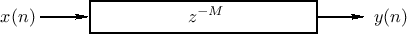
\includegraphics[scale=0.5]{Pictures/delayline.png}
	\caption{An M-sample delay line}
	\label{fig:delayline}
\end{figure}

\subsection*{Digital waveguides}
A digital waveguide is defined as a bidirectional delay line (fig \ref{fig:waveguide}) representing two traveling waves in opposite directions. When exciting an ideal string, we can decomposed the movement into two such traveling waves. Such system is useful for one-dimensional acoustic system (strings or wind instruments)
\begin{figure}
	\centering
	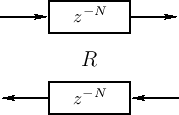
\includegraphics[scale=0.5]{Pictures/waveguide.png}
	\caption{A digital waveguide $N$ sample long}
	\label{fig:waveguide}
\end{figure}

Excitations of such a system is specified by providing an input to both delay lines (for example, a Dirac impulse). Output are handle by adding up both signals.\\
Such a model can be used to describe an ideal string.

\subsection*{Terminations}
The last element to take into account to describe one-directional instruments are the ends or the system. At those terminations the string don't move and the wave is reflected by either a coefficient (less than 1 to attenuate the signal) or a specific filter to model such a termination.

\begin{figure}
	\centering
	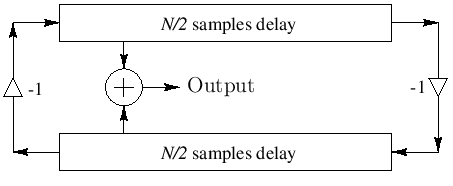
\includegraphics[scale=0.5]{Pictures/terminations.png}
	\caption{Rigidly terminated string}
	\label{fig:terminations}
\end{figure}

\section{The Faust language}

Faust (Functional Audio Stream) is a functional programming \cite{quickref} language designed for real-time signal processing and synthesis. It provides an adequate notation to describe signal processors and thus to quickly develop audio programs, along with block-diagram algebra.

\subsection*{Syntax}

A Faust program contains a "main" function called \texttt{process} that consists in a signal processor.
Signal processors take input signals and give output signals: \texttt{process(x) = x;} (identity). Common operators are usable in Faust (\texttt{+, -, *, /, mod}). The identity function can also be specified with the operator : \texttt{process = \_;}.\\
Block diagram compositions can be handle with common operations as parallel composition \texttt{,}, sequential composition \texttt{:}, split composition \texttt{<:}, merge composition \texttt{:>} and the recursive composition \texttt{~}. The \texttt{~} operator stands for recursive composition : \texttt{process = + \~ \_;}. If x is the input, that block features the equation $y(n) = x(n) + y(n-1)$ (see figure \ref{fig:recursive}).
For those operations, number of inputs and ouputs has to be taken with care.
\begin{figure}[h]
	\centering
	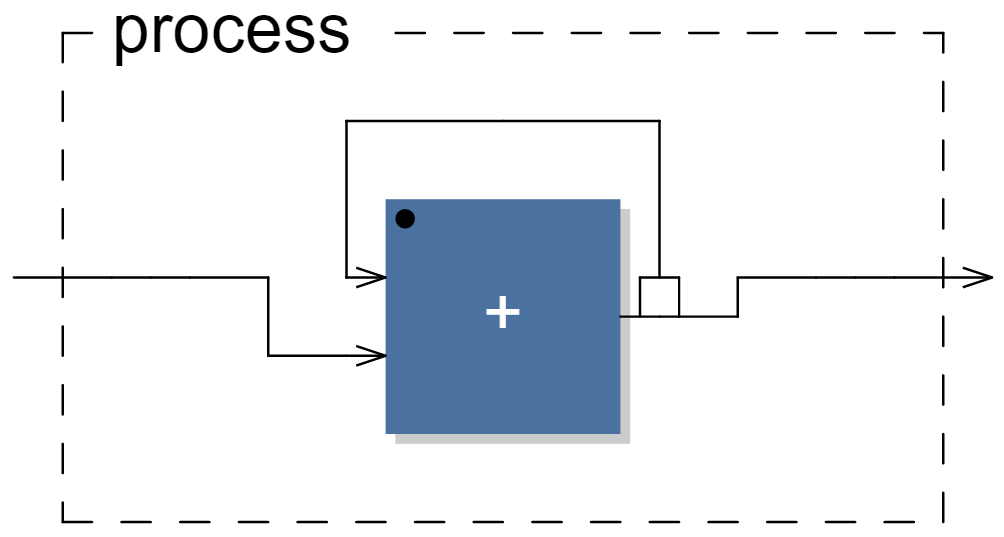
\includegraphics[scale=0.2]{pictures/recursive.png}
	\caption{Block diagram generated for the code \texttt{process = + \~ \_}}
	\label{fig:recursive}
\end{figure}

\subsection*{Diagrams generation}
That kind of diagram is very handy to generate using the command line with \texttt{faust -svg myprocessor.dsp}. This tools shows the powerful of Faust which enables a musician to quickly build sound effects or instruments.

\subsection*{Libraries}
As most of programming languages, Faust comes with the possibility to import libraries, which are \texttt{.lib} files : \texttt{import("math.lib");}. As useful libraries, we can name \texttt{math.lib} (common math operations), and more signal processing oriented libraries as \texttt{music.lib} (spatialisation, envelops, delays, etc.) and \texttt{filter.lib} (digital filters) \cite{filters}


\section{Physical modeling library pm.lib}

The Faust language as it is specified for now allows to generate only one-directional diagram blocks, from left (inputs) to right (outputs), so a bidirectional delay lines can't be achieved as in fig \ref{fig:waveguide}. That issue has been circumvented with a \texttt{chain} function that takes both input to the left (+ one extra input) and gives both outputs to the fight (+ one extra output to mix both signals), as shown in diagram \ref{fig:chain}. One main issue of this circumvent is that it adds a one-sample delay to the signal.

\begin{figure}[h]
	\centering
	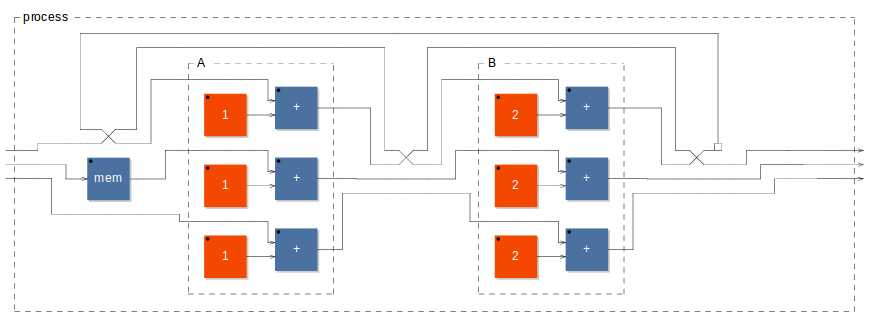
\includegraphics[scale=0.3]{pictures/chain.png}
	\caption{Use of chain(A:B) where \texttt{A=+1,+1,+1} and \texttt{B=+2,+2,+2}}
	\label{fig:chain}
\end{figure}

 The \texttt{chain} function can be more easily seen as adding up bidirectional blocks one after another as in figure \ref{fig:chainrepresentation}.

\begin{figure}[h]
	\centering
	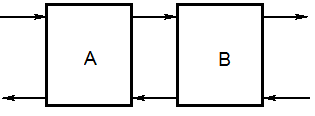
\includegraphics[scale=0.5]{pictures/chainrepresentation.png}
	\caption{The \texttt{chain} aims to put blocks in succession.}
	\label{fig:chainrepresentation}
\end{figure}

This basic component \texttt{chain} comes along with termination component and excitation functions. The terminations are based on a generic \texttt{terminations} (letting chains opened) to give \texttt{fullTerminations} (it closes chains), and \texttt{leftTermination} and \texttt{rightTermination} (they close only one end). Functions as a Dirac impulse and a noise burst \cite{lac_orlarey} has been written to excite instruments.\\

Finally we are equipped to build our first physical modeling based instrument : an ideal string. First the \texttt{waveguide} model is written using a $4^{th}$ order fractional delay for each delay line with a \texttt{n} samples length : \texttt{waveguide(nMax,n) = fdelay4(nMax,n),fdelay4(nMax,n),\_;}\\
An ideal string is then written as :
\texttt{idealString(length,reflexion,pluckPosition,x) = fullTerminations(term,wg,term)
	with\{...\};	
} where we specify the string length, the reflexion coefficient (or filter) and the pluck position (0-0.99), \texttt{wg} being the previous \texttt{waveguide} function, and \texttt{term} calcultated with the given parameters. \texttt{x} is the input of the system (excitation function).
This \texttt{idealString} function led to other functions like \texttt{steelString} and \texttt{nylonString} where the reflection coefficient of -1 had been replaced by a damping filter designed by ear to sound the most accurately possible.

\section{IR2dsp.py and mesh2dsp.py scripts}

Those two scripts were written  for the same goal: to recreate the sound of an object when stricking by an small impulse. With a functional and powerful algorithm, it would be possible to model any object vibration sound which lead to many musically beautiful possibilities.

\subsection*{IR2dsp.py}

IR2dsp.py is a python script which aim to recreate the sound of a stricking object, giving its impulse response (IR) in input. It outputs a filterbank model of the object written in a Faust \texttt{.dsp} file.\\
The algorithm is divided into several step. First, a Fourier Fast Transform (FFT) realised to compute the power spectrum or the IR. Then we detect frequency peaks in the data provided by the FFT, with information from input parameters such as minimum frequency threshold and minimum peak distance. The algorithm then analyzes each detected peak to calculate the width of each one.\\
Finally the script had been able to calculate three parameters to describe each peak : the centrale frequency, the value of the peak (the gain in dB) and the width which is transformed into audio decay time.\footnote{see https://ccrma.stanford.edu/~jos/mdft/Audio\_Decay\_Time\_T60.html}. Each triplet of parameters describes a bandpass filter of the shape of the corresponding peak. Finally put together, this gives a filterbank of bandpass filters (see fig \ref{fig:filterbank}) that recreate at a certain accuracy the sound of the corresponding object when excitated.

\begin{figure}[h]
	\centering
	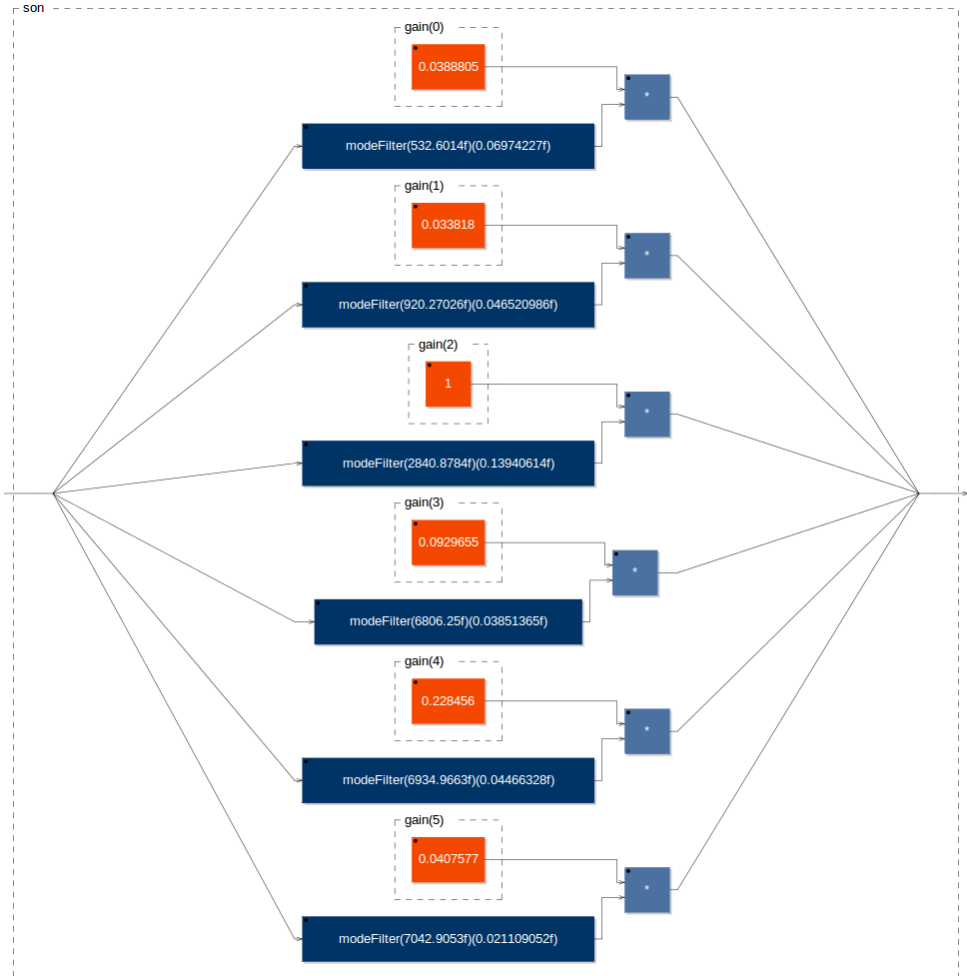
\includegraphics[scale=0.2]{pictures/filterbankdiagram.png}
	\caption{Diagram of a filterbank generated with a glass IR}
	\label{fig:filterbank}
\end{figure}

\subsection*{mesh2dsp.py}

This second script aims to generate the same result : the creation of a filterbank model written in Faust in order to recreate the sound of a vibrating object.\\
Given a geometric file (\texttt{.stl} file) specifying the shape of an object, the script perform a finite element analysis (FEA) with the open-source software Elmer.\footnote{https://www.csc.fi/web/elmer} Three parameters has to be given for the FEA as inputs of the script : the Young modulus, the Poisson coefficient and the density of the material of the object.\\
The algorithm extracts from the FEA output the computed eigen values that are tranformed into frequencies. With those frequencies, we are able to generated the previously explained filterbank model, except that we do not have two parameters : the power of each filter (gain in dB) and the audio decay time. The audio decay time cannot be compute from a FEA. The gains of each vibration frequencies can be retrieved from the FEA but unfortunately the documentation and ressources for Elmer did not allow us to find this out.\\
Another difficulty of this method is that, during the FEA, we need to precise some immobility constraints (e.g. both ends of a string), which makes the algorithm less automated.

\section{Conclusions}

We presented the work that has been begun on a physical modeling library in the Faust audio language. We gave a quick tour of what is physical modeling synthesis, then a quick review of the manner to write audio programs in Faust. We introduced the library by pointing out that Faust is not fully operationnal for physical modeling in its present form, then the basis of the library was explained with the first sounding pieces of instrument. We finally presented two scripts of which goal is very interesting, but with some limitation especially with the FEA.\\

Future works will focus on proposing more instrument elements to provide a modular audio library to construct instruments pieces by pieces. The first presented script works well but the second one should be rethought from the beginning as the FEA analysis had given us hard time.

\section{Acknowledgements}

Our thanks go to \ldots .

\bibliographystyle{acl}
\bibliography{sample}

\end{document}
